\documentclass{article}
\usepackage{blindtext}

% spanish language
\usepackage{graphicx,dblfloatfix}
\usepackage[margin=1.5in]{geometry}
\usepackage{subfigure} % subfiguras
\usepackage{multicol}% http://ctan.org/pkg/multicols
\usepackage{lipsum}% http://ctan.org/pkg/lipsum
\usepackage[utf8]{inputenc}
\usepackage[spanish]{babel}
\usepackage{titlesec}

% links
\usepackage{hyperref}
\hypersetup{
    colorlinks=true,
    linkcolor=blue,
    filecolor=magenta,
    urlcolor=blue,
}

\usepackage{bibentry}

\hyphenation{op-tical net-works semi-conduc-tor}

\begin{document}
%
% paper title
% can use linebreaks \\ within to get better formatting as desired
\title{Análisis de datos sobre películas, sus metadatos y premios}

\author{Javier~Pozueco,~Technical~Analytics~Director,~Jellyfish,% <-this % stops a space
}

% make the title area
\maketitle

\providecommand{\keywords}[1]{\textbf{\textit{Keywords:}} #1}

\begin{abstract}
%\boldmath
\blindtext[1]
% Note that keywords are not normally used for peerreview papers.
\\
\\
\begin{keywords}
IMDb, Kaggle %IEEEtran, journal, \LaTeX, paper, template.
\end{keywords}
\end{abstract}

\section{Introducción y objeto del análisis}

\blindtext

\blindtext

\clearpage

\section{Carga de los datos y análisis descriptivo}
Existen multitud de bases de datos de libre disposición con información general relacionada con películas. Una de estas bases de datos es La Internet Movie Database (o IMDb de manera abreviada), que muestra toda su informacion a través del portal web \href{http://www.imdb.com}{http://www.imdb.com}.

Para esta base de datos en particular, el usuario tiene acceso al título de las películas, el nombre del director, las personas que han participado en su realización, el genéro, su presupuesto o el dinero recaudado, como se puede ver a continuación:

\begin{figure}[h]
\centering
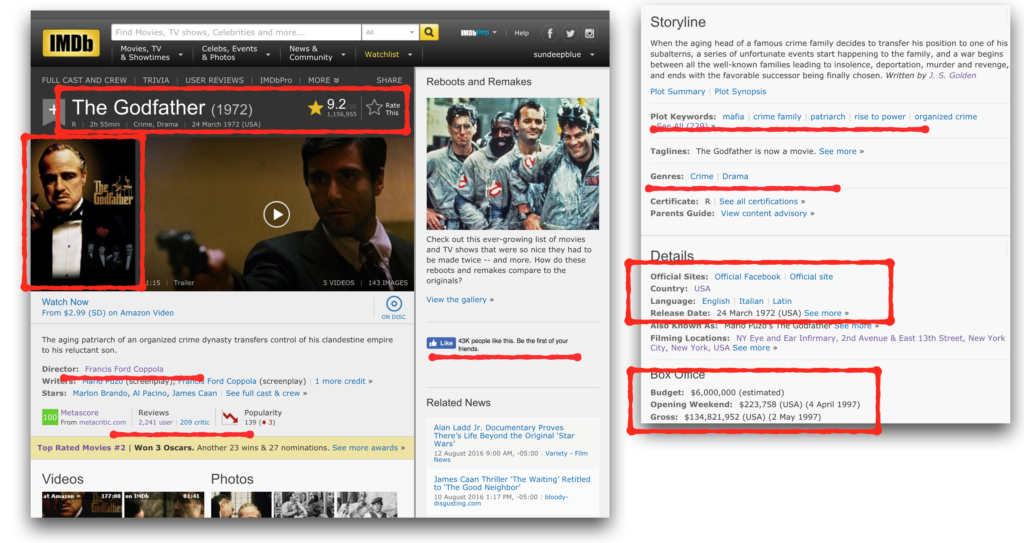
\includegraphics[width=3in,clip,keepaspectratio]{./images/imdb_data}
\label{fig:imdb_data}
\end{figure}

A pesar IMDb sólo presenta su información a través de su portal web, hay trabajos como \cite{imdb5000} que ya han extraído los datos más relevantes utilizando, en este caso en particular, Python y su librería \href{https://scrapy.org/}{scrapy}, siguiendo los siguientes pasos:

\begin{itemize}
  \item Se ha utilizado scrapy para obtener un listado de 5043 películas desde el portal \href{http://www.the-numbers.com/movie/budgets/all}{The Numbers}.
  \item Se ha realizado una búsqueda en IMDb para obtener el enlace a cada una de las películas.
  \item Para cada uno de los enlaces, se ha descargado y parseado su contenido, con el fin de obtener los datos más relevantes que se pueden ver en la siguiente figura:

    \begin{figure}[h]
    \centering
    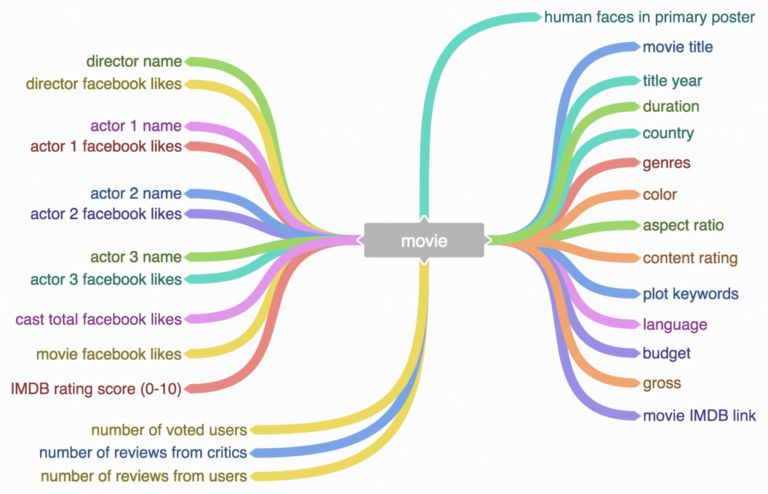
\includegraphics[width=3in,clip,keepaspectratio]{./images/imdb_attributes}
    \label{fig:imdb_attributes}
    \end{figure}

  \item Mediante el reconocimiento de imágenes, también se sabe para cada película el número de caras que aparecen en su póster.
\end{itemize}

A continuación se incluyen notas importantes del autor, sobre cada uno de los atributos extraídos de las películas, que deberemos  tener en cuenta en el análisis que se realizará más adelante:

\begin{itemize}
  \item En aproximadamente 800 películas las ganacias son 0, debido a que esta información no está disponible o porque la herramienta utilizada para extraer el dato no devolvió ninguna respuesta en un tiempo razonable.
  \item En 908 directores de las películas descargadas, el número de likes en Facebook es 0 debido, como en el caso anterior, a que los valores aparecen en un marco que no se carga junto con el resto de la página.
  \item Hay películas para las que no se ha tenido en cuenta la moneda del país que las ha producido, y aunque en los datos se muestran dólares, en realidad es la moneda del país correspondiente.
  \item Para calcular los actores principales de cada película, se han tenido en cuenta todos los actores y actrices del reparto, y aquellos tres con mayor número likes en Facebook, son considerados los principales.
  \item Por último, cabe destacar también que el presupuesto y las ganancias de las películas no tienen en cuenta la inflación o el cambio de moneda que había en el año de su realización.
\end{itemize}

%\clearpage

\subsection{Datos generales sobre el dataset}

Como primer paso vamos a analizar el dataset extraído de \href{https://www.kaggle.com/deepmatrix/imdb-5000-movie-dataset}{Kaggle}, que será el utilizado en este trabajo. Para ello se muestra en la siguiente figura el número de películas por país en nuestro dataset cada año disponible en \href{https://public.tableau.com/profile/javier6580\#!/vizhome/proyecto_fin_de_master_dataset/films_per_year}{Tableau Public}:

\begin{figure}[h]
\centering
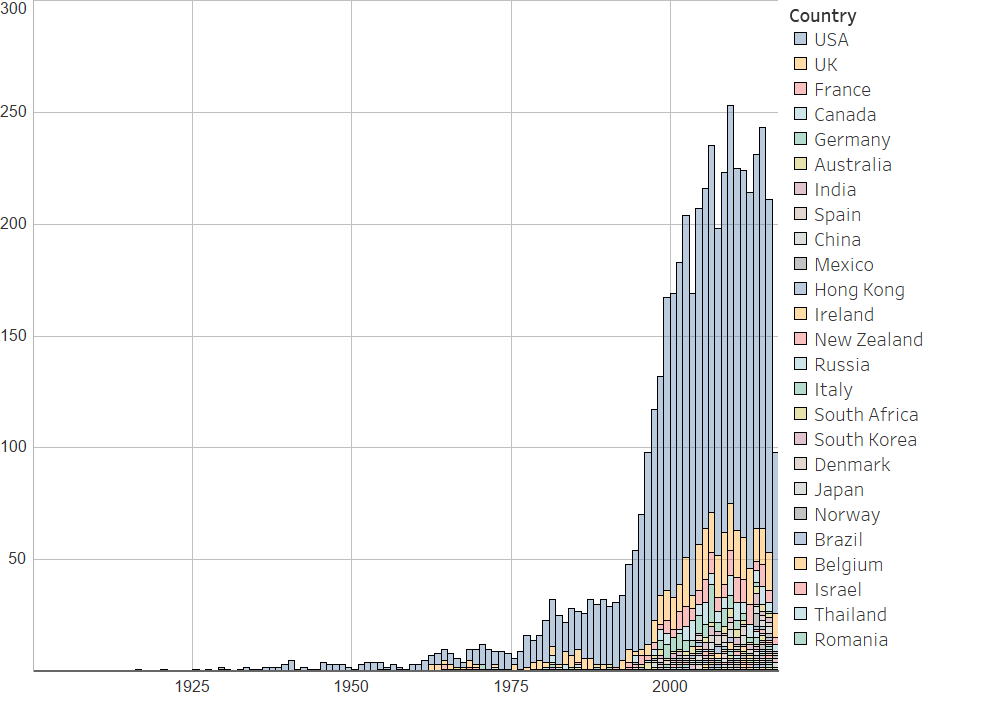
\includegraphics[width=4.5in,clip,keepaspectratio]{./images/films_per_year.png}
\label{fig:kaggle_num_films_per_year}
\end{figure}

A continuación se muestra el número total de películas, incluyendo también series, según IMDb\cite{quora}. El número de películas descargado resulta ser inferior al 3\% del total, pero al ser un listado con los datos disponibles en \href{http://www.the-numbers.com/movie/budgets/all}{The Numbers}, podemos considerar que son las que tienen ganancias conocidas y mayores:

\begin{figure}[h]
\centering
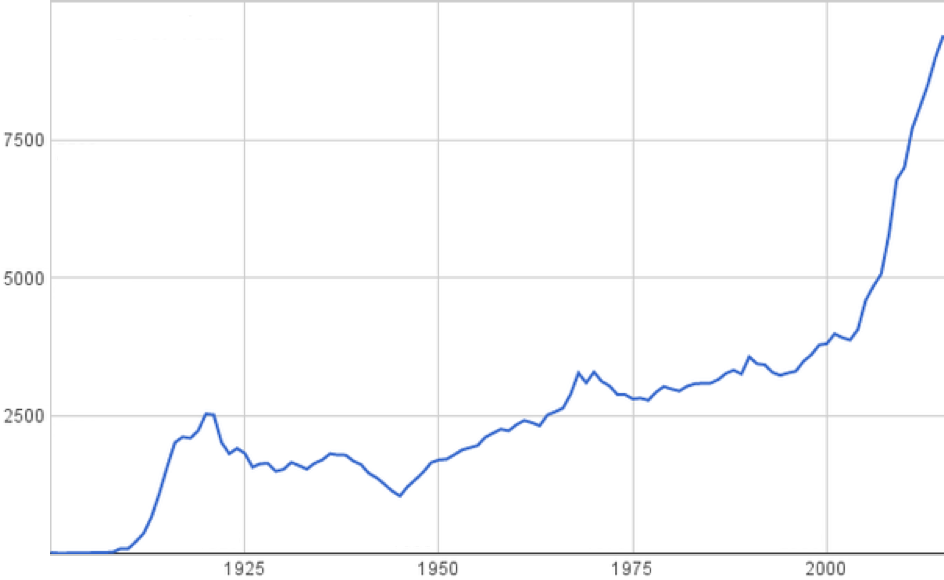
\includegraphics[width=3.3in,clip,keepaspectratio]{./images/total_movies_imdb}
\end{figure}

\subsection{Rating otorgado por los usuarios}

En el listado de películas considerado se incluye también el rating otorgado por los usuarios según IMDb. Este valor proviene de las puntuaciones que dan los usuarios con valores comprendidos entre 0 y 10, y que a través de diferentes métodos se pondera para evitar que un mismo usuario pueda votar varias veces.

Para que una película pueda estar dentro del top 250 de IMDb sólo se tienen en cuenta las votaciones de los usuarios más frecuentes, aunque para evitar cualquier tipo de engaño los requisitos necesarios para ser un usuario frecuente no se han publicado:

\begin{equation}
W=\frac{R_{v}+C_{m}}{v+m}
\end{equation}

\noindent
donde:\\

\indent
$W$ = rating ponderado\\
\indent
$R$ = media de las votaciones de 0 a 10\\
\indent
$v$ = número de votos\\
\indent
$m$ = mínimo número de votos para estar en el top 250\\
\indent
$C$ = la media de todos los votos\\

En la figura que se muestra a continuación se puede observar la distribución del rating otorgado por los usuarios en el dataset considerado. En este gráfico se han destacado las películas según su calidad, en base a los siguientes criterios disponible en \href{https://public.tableau.com/profile/javier6580\#!/vizhome/proyecto_fin_de_master_dataset/rating_distribution}{Tableau Public}:

\begin{itemize}
  \item Verde, si las películas son muy buenas y superan una puntuación de 8.
  \item Amarillo, si las películas son buenas y tienen una puntuación entre 6,5 y 8.
  \item Naranja, si las películas son regulares y tienen una puntuación entre 5 y 6,5.
  \item Rojo, si las películas son malas y bajan del 5.
\end{itemize}

\begin{figure}[h]
\centering
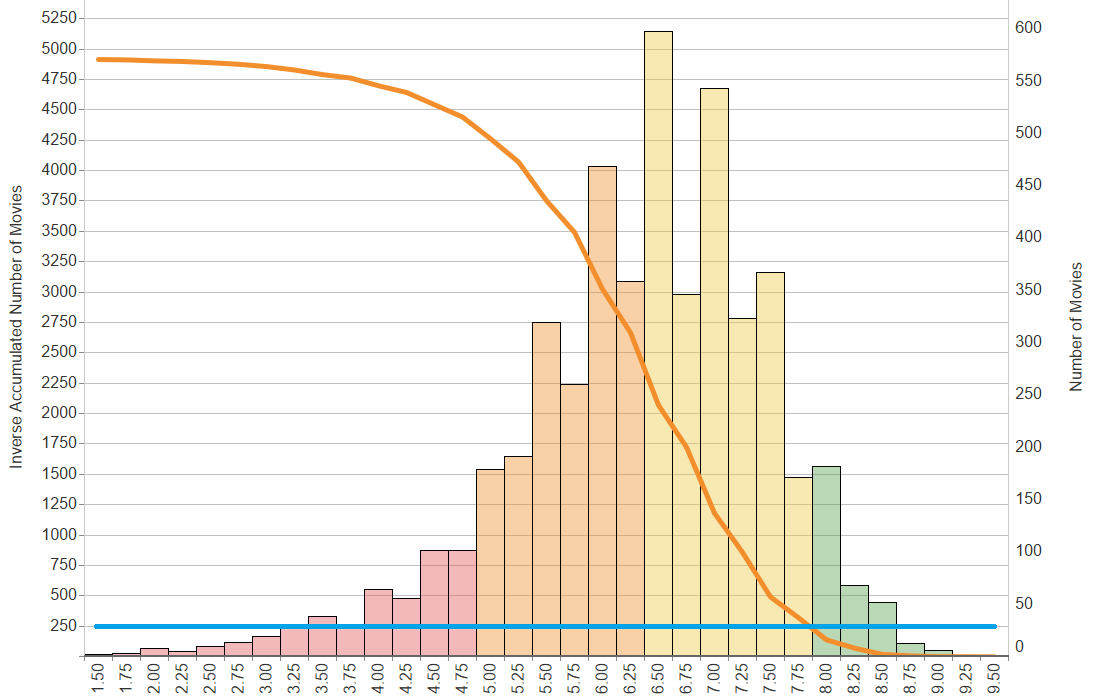
\includegraphics[width=4in,clip,keepaspectratio]{./images/rating_distribution}
\label{fig:imdb_rating_distribution}
\end{figure}

Cabe destacar también como el top 250 de IMDb se corresponde con una puntación ligeramente inferior a 8, según el gráfico anterior.

\subsection{Distribucion de las puntuaciones}

Desde finales de la segunda guerra mundial, se ha producido un incremento gradual de las películas producidas debido al avance de la tecnología para la realización de las mismas. Además, como se pudo ver anteriormente en el número de películas producidas cada año, desde finales del siglo pasado el avance de los medios digitales ha facilitado y abaratado su distribución para multitud de productoras independientes\cite{popmatters}. Por otro lado, en la siguiente figura también se puede observar que aunque el número de trabajos ha aumentado, también ha dismunido la calidad en algunos casos disponible en \href{https://public.tableau.com/profile/javier6580\#!/vizhome/proyecto_fin_de_master_dataset/rating_year}{Tableau Public}:

\begin{figure*}[h]
\centering
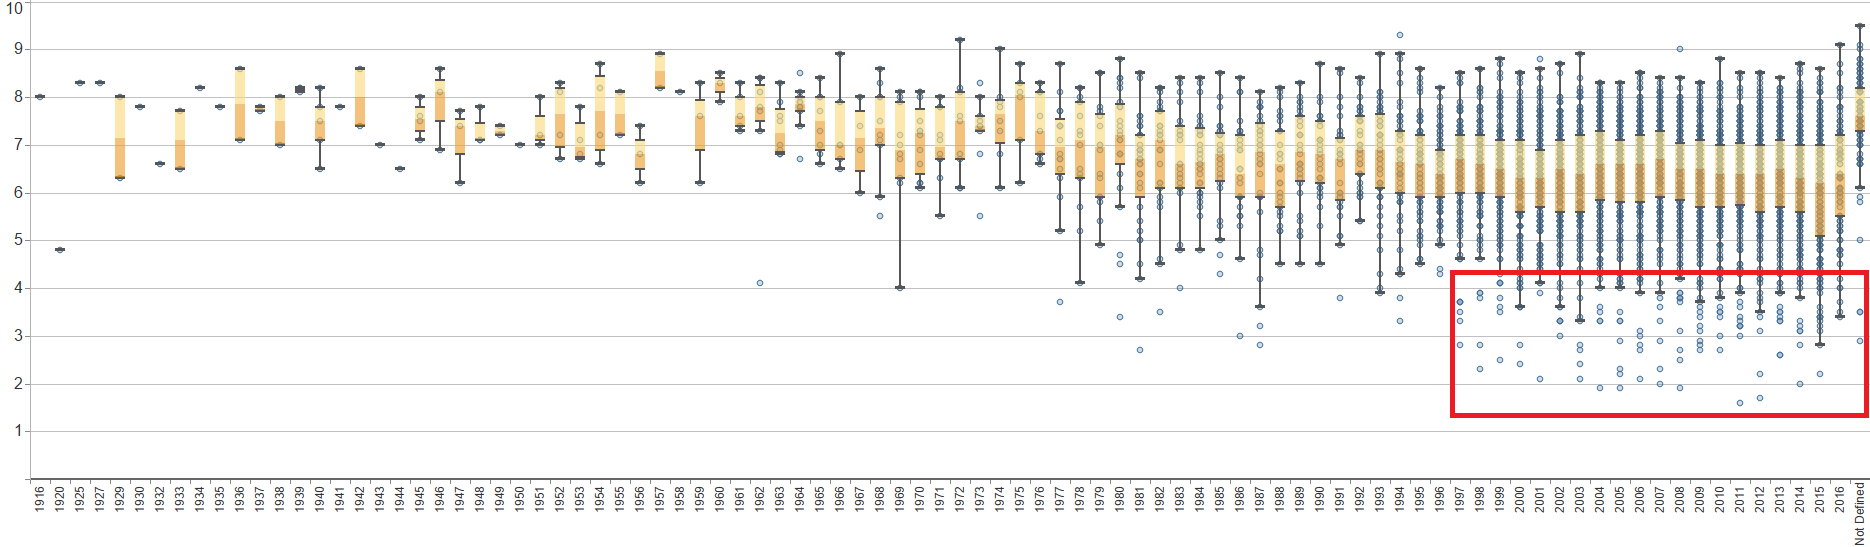
\includegraphics[width=\textwidth,keepaspectratio]{./images/rating_year}
\end{figure*}

\clearpage

Hay países como Kirguistán, Libia, Egipto o Irán con un reducido número de películas pero cuya puntuación es superior al resto. Por otro lado Estados Unidos, Reino Unido y Francia son los países con más películas, pero cuya calidad no siempre es mejor que las demás. Cabe destacar que en el dataset que estamos estudiando aparecen películas de la India pero no en gran cantidad, siento este país uno de los productores actuales más grande disponible en \href{https://public.tableau.com/profile/javier6580\#!/vizhome/proyecto_fin_de_master_dataset/rating_country}{Tableau Public}:

\begin{figure*}[h]
\centering
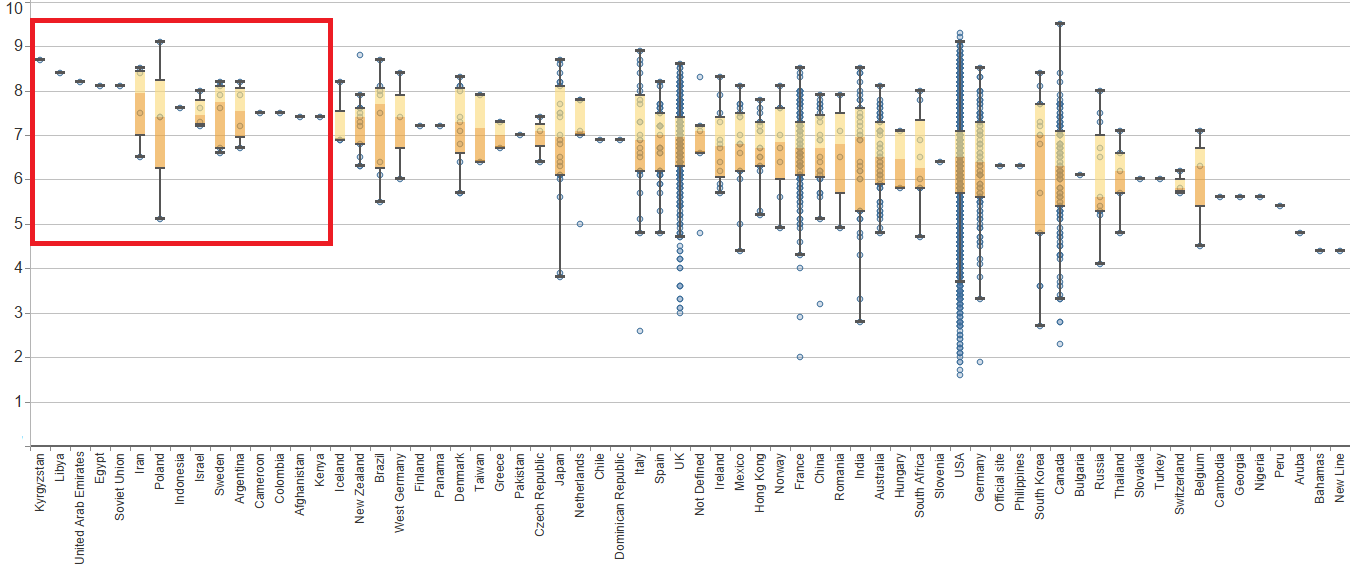
\includegraphics[width=\textwidth,keepaspectratio]{./images/rating_country}
\end{figure*}

\subsection{Análisis de actores y directores}

Resulta interesante también analizar las puntuaciones de los actores y directores con mayor número de películas. Se puede ver a continuación como la variación de las puntuaciones de los actores es mayor que la de los directores más populares. En el caso de los actores, algunos nombre como Robert De Niro, Sylvester Stallone o Channing Tatum con buenas películas, pero también con películas de calidad mediocre. Otros actores como Matt Damon destacan por tener un gran número de películas de calidad notable y Nicolas Cage, por ejemplo, por haber realizado algunos papeles de mala calidad. Con respecto a los directores destaca Steven Spielberg como el actor mas prolífico y siempre de gran calidad y Robert Rodríguez con diferentes producciones pésimas disponible en \href{https://public.tableau.com/profile/javier6580\#!/vizhome/proyecto_fin_de_master_dataset/rating_actors}{Tableau Public 1} y \href{https://public.tableau.com/profile/javier6580\#!/vizhome/proyecto_fin_de_master_dataset/rating_directors}{Tableau Public 2}.

\begin{figure}[h]
\centering
\subfigure[Actores más populares]{
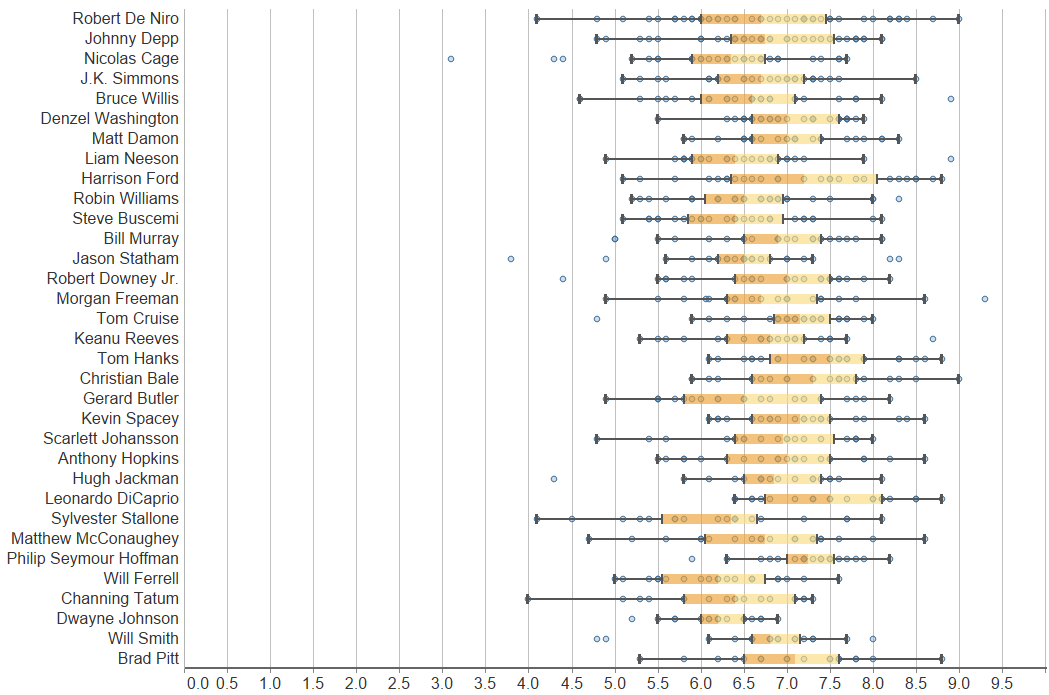
\includegraphics[width=2.6in]{./images/rating_actors}
}
\subfigure[Directores más populares]{
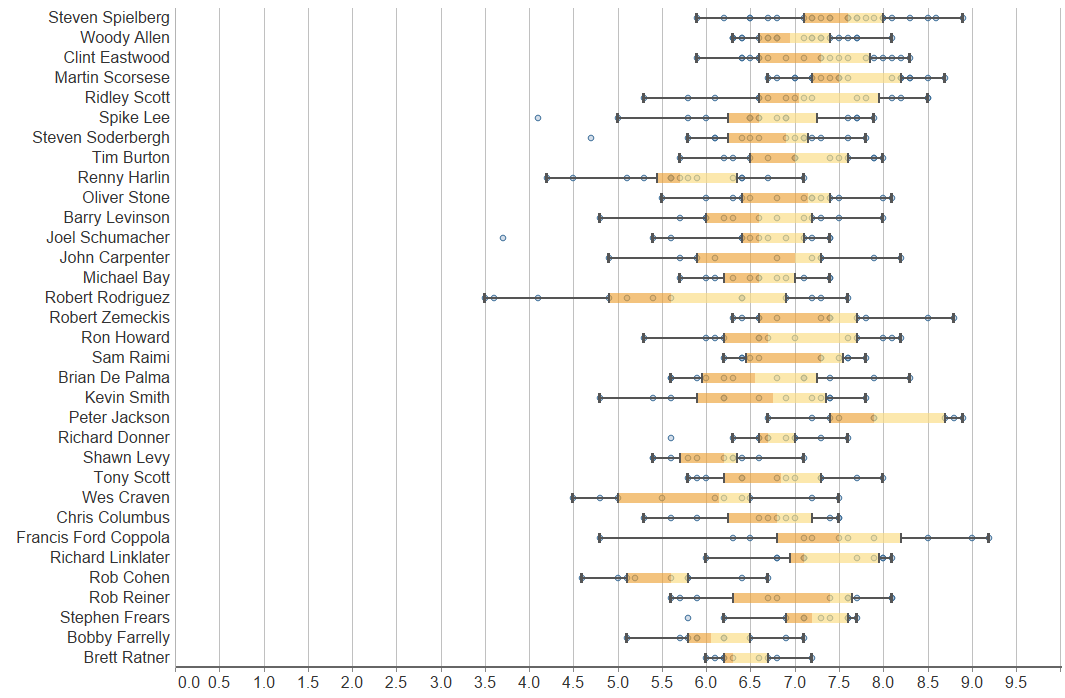
\includegraphics[width=2.6in]{./images/rating_directors}
}
\end{figure}

\clearpage

Para saber si influye el número de likes en la puntuacíon de las películas, podemos ver en los siguientes gráficos como es más importante en los actores tener más likes para obtener mejores resultados, y sobre todo el en actor principal de la película, pero en los directores aunque con menos likes, las puntuaciones son superiores disponible en \href{https://public.tableau.com/profile/javier6580\#!/vizhome/proyecto_fin_de_master_dataset/likes_actors_rating}{Tableau Public 1} y \href{https://public.tableau.com/profile/javier6580\#!/vizhome/proyecto_fin_de_master_dataset/likes_director_rating}{Tableau Public 2}:

\begin{figure}[h]
\centering
\subfigure[Número de likes de los actores]{
\centering
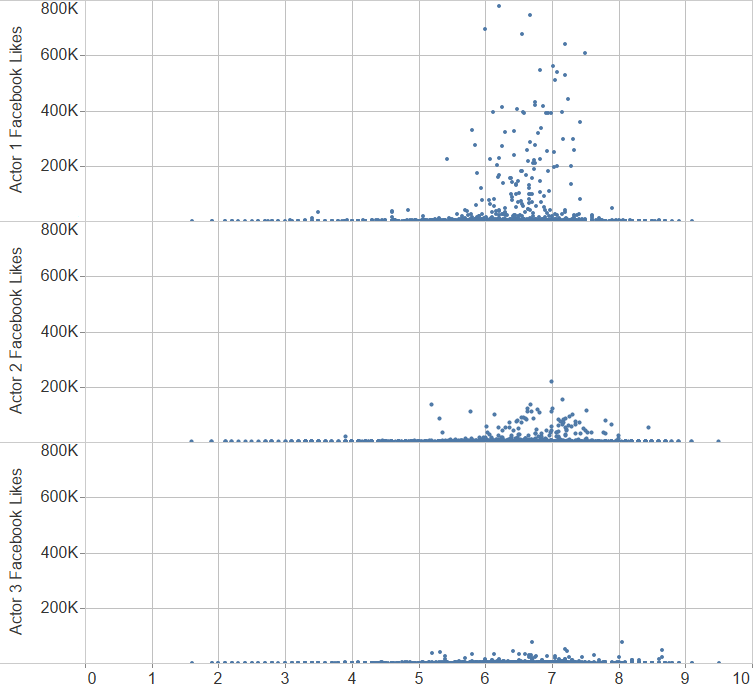
\includegraphics[width=2.6in]{./images/likes_actors_rating}
}
\subfigure[Número de likes de los directores]{
\centering
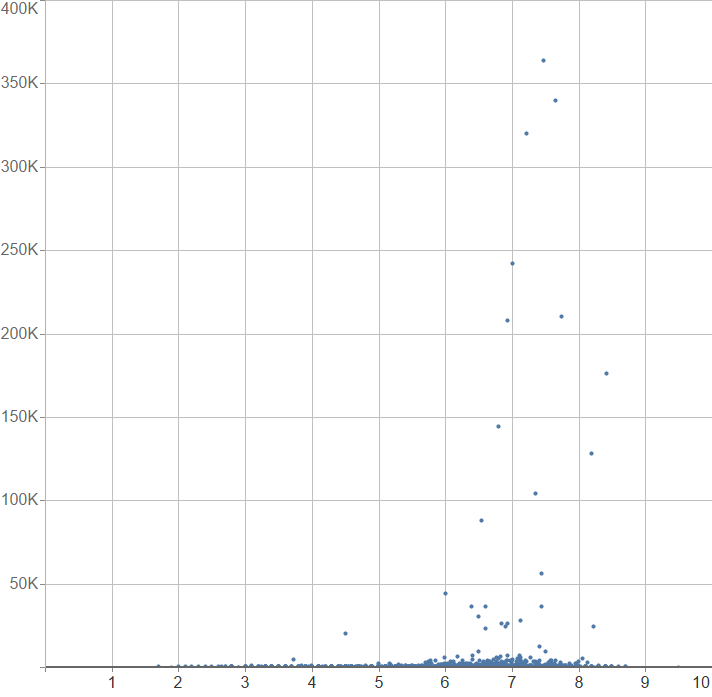
\includegraphics[width=2.6in]{./images/likes_director_rating}
}
\end{figure}

%\clearpage

\subsection{Análisis de presupuesto y duración}

Para saber si influye el presupuesto y la duración de las películas en la puntuación obtenida en IMDb, se puede ver como a mayor dinero invertido menor es la dispersión en las puntuaciones, y aquellas películas que son mejores tienen una duración de menos de una hora o de longitud más larga posible disponible en \href{https://public.tableau.com/profile/javier6580\#!/vizhome/proyecto_fin_de_master_dataset/rating_budget}{Tableau Public 1} y \href{https://public.tableau.com/profile/javier6580\#!/vizhome/proyecto_fin_de_master_dataset/rating_budget}{Tableau Public 2}:

\begin{figure}[h]
\centering
\subfigure[Rating por presupuesto]{
\centering
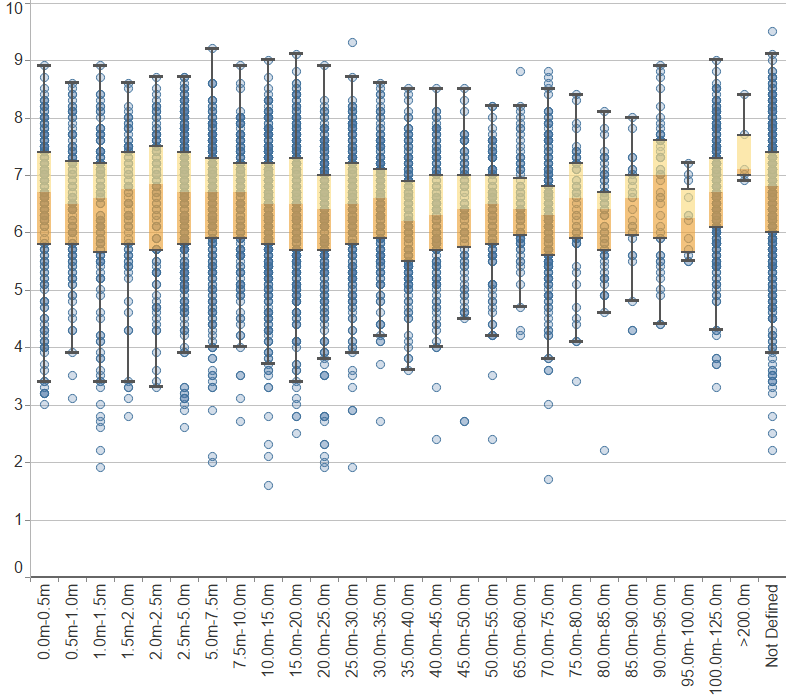
\includegraphics[width=2.6in]{./images/rating_budget}
}
\subfigure[Rating por duración]{
\centering
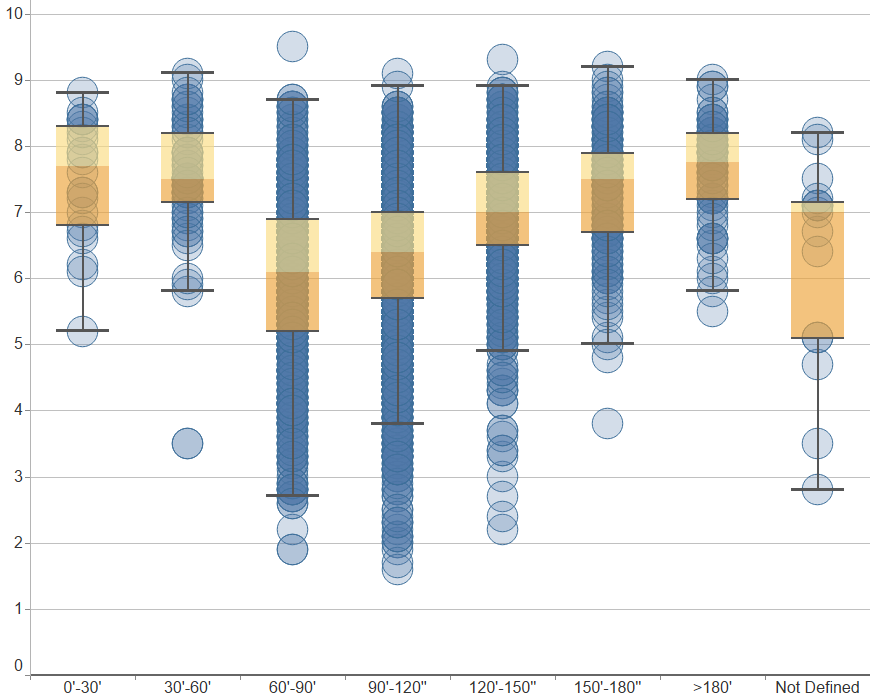
\includegraphics[width=2.6in]{./images/rating_duration}
}
\end{figure}

\clearpage

La combinación de estos dos factores nos muestra que una gran duración y presupuesto moderado resulta en mejores películas y como las películas de entre media hora y una hora también tienen gran aceptación entre el público disponible en \href{https://public.tableau.com/profile/javier6580\#!/vizhome/proyecto_fin_de_master_dataset/budget_duration}{Tableau Public}:

\begin{figure}[h]
\centering
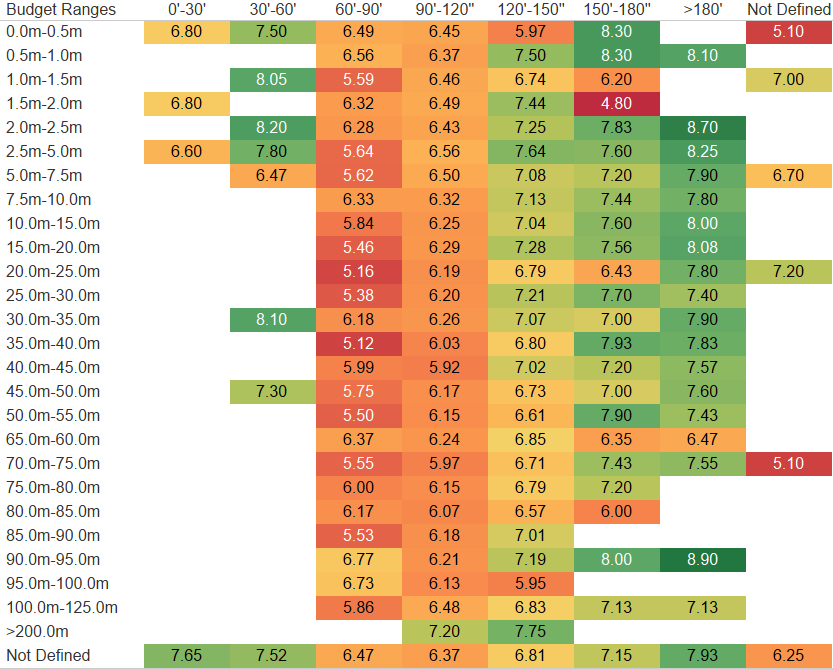
\includegraphics[width=4in,clip,keepaspectratio]{./images/budget_duration}
\end{figure}

Como curiosidad se puede ver como ha variado la duración de las películas a lo largo del tiempo\cite{justgeek}, podemos representar los ragos de duración anualmente y ver como son cada vez más populares las películas con una duración de entre 90 y 120 minutos disponible en \href{https://public.tableau.com/profile/javier6580\#!/vizhome/proyecto_fin_de_master_dataset/duration_year}{Tableau Public}:

\begin{figure}[h]
\centering
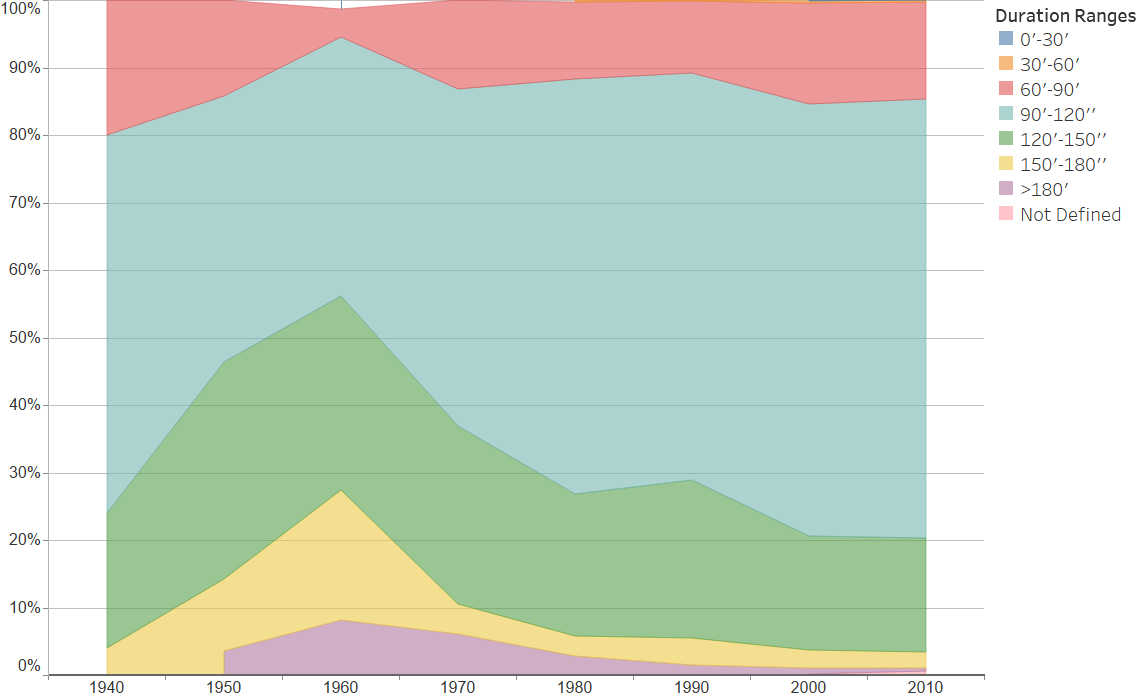
\includegraphics[width=4in,clip,keepaspectratio]{./images/duration_year}
\end{figure}

%\clearpage

\clearpage

\subsection{Análisis del género de las películas}

Para saber si el género de las películas influye en el rating de las mismas se muestra a continuación como aquellos generos menos populares son los que mayor puntuación reciben y el drama, que es el género más popular, se situa tras de estos, disponible en \href{https://public.tableau.com/profile/javier6580\#!/vizhome/proyecto_fin_de_master_dataset/rating_genre}{Tableau Public} y el script utilizado para dividir el género en \href{https://github.com/pozueco/proyecto_fin_de_master/blob/master/split_genres.md}{R Markdown}:

\begin{figure}[h]
\centering
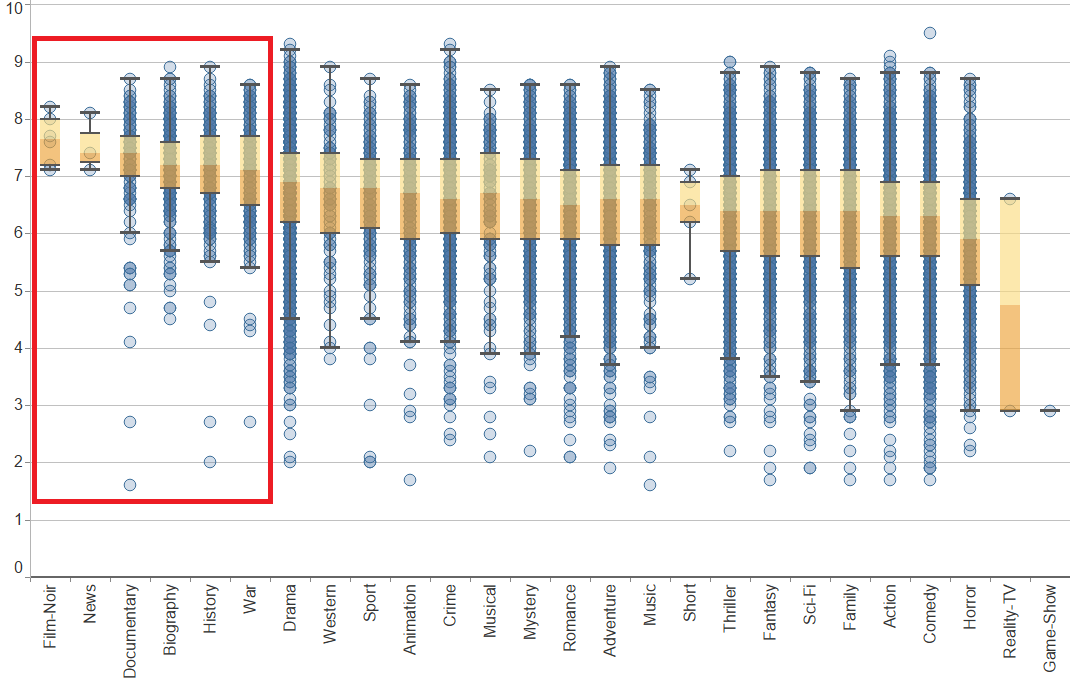
\includegraphics[width=4.5in,clip,keepaspectratio]{./images/rating_genre}
\end{figure}

Es interesante también ver como han evolucionado los géneros más populares a lo largo del tiempo, para ver como la acción, el thriller o la comedia son cada vez más populares y otros como el drama y el romance, ya no tanto, disponible en \href{https://public.tableau.com/profile/javier6580\#!/vizhome/proyecto_fin_de_master_genre/rating_genre}{Tableau Public}:

\begin{figure}[h]
\centering
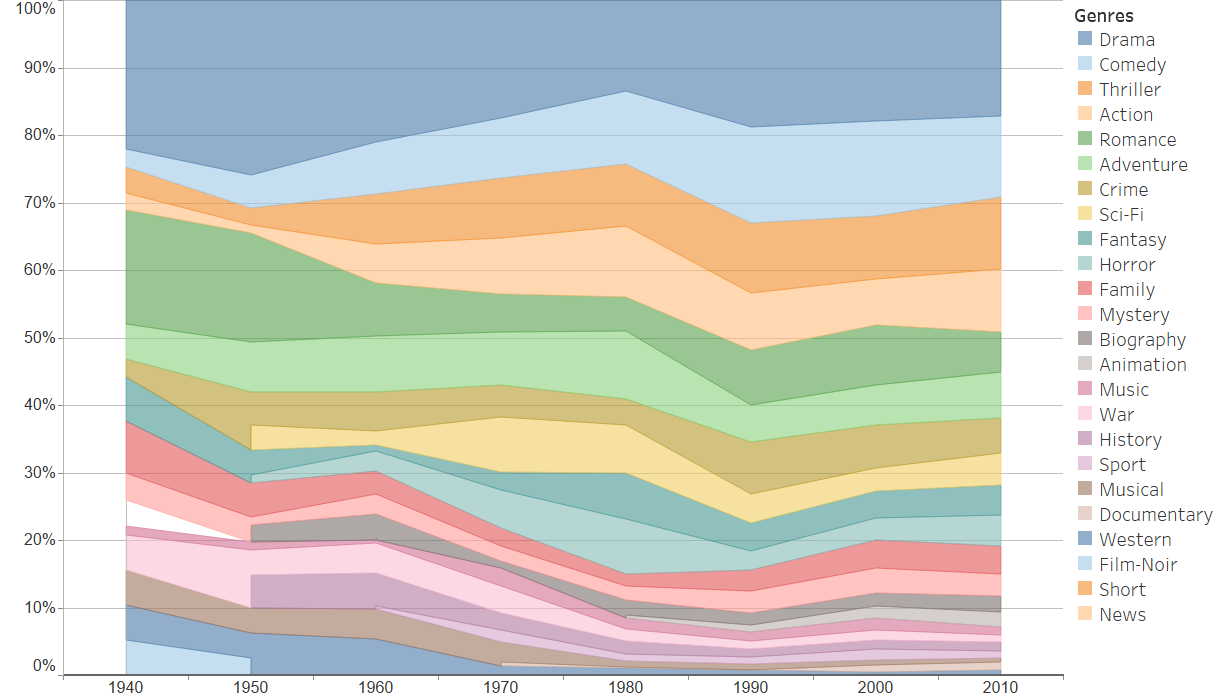
\includegraphics[width=4.5in,clip,keepaspectratio]{./images/genre_year}
\end{figure}

\clearpage

\section{Preparación y limpieza del dataset}

En primer lugar se ha realizado un análisis de la calidad del dataset para saber la cantidad de datos no disponible para cada uno de los atributos. Como se puede ver en el anexo \ref{anexo:I}, el presupuesto de las películas y las ganancias en mayor medida, arrojan una mayor falta de datos que el resto de características del dataset. Como las ganancias es un dato conocido únicamente despues de haberse realizado la película, no será tenido en cuenta en la creación de los modelos detallados en la siguientes secciones. 

\subsection{Modelo no supervisado}

A continuación se seleccionan los datos para la construcción del modelo no supervisado solamente con las siguientes columnas, y se eliminan las files con datos no definidos con \href{https://github.com/pozueco/proyecto_fin_de_master/blob/master/clean_dataset.md}{R Markdown}:

\begin{itemize}
  \item Actor 1 Facebook Likes, Actor 2 Facebook Likes y Actor 3 Facebook Likes 
  \item Director Facebook Likes
  \item Duration
  \item Budget
\end{itemize}

\subsection{Modelo supervisado}

Para la construción de los modelos de regresión se utilizarán las siguientes columnas y eliminándose como en el caso anterior las files con datos no definidos con \href{https://github.com/pozueco/proyecto_fin_de_master/blob/master/clean_dataset.md}{R Markdown}. Cabe destacar que se ha creado una columna por género de la película con el valor 0 o 1 si la película pertenece a ese género, una columna con el valor 0 o 1 si la película es el blanco y negro o en color, y una columna para el director, el actor 1, el actor 2 y el actor 3, con el número de películas en las que participan:

\begin{itemize}
  \item Actor 1 Facebook Likes, Actor 2 Facebook Likes y Actor 3 Facebook Likes
  \item Director Facebook Likes
  \item Duration
  \item Budget
  \item Title Year
  \item Face Number in Poster
  \item Number Critic for Reviews
  \item Color
  \item Genre
  \item Director Movies
  \item Actor 1 Movies, Actor 2 Movies y Actor 3 Movies
  \end{itemize}

\clearpage

\subsection{Recomendador}

\blindtext

\clearpage

\section{Análisis exploratorio apoyado en algún método NO supervisado}

Para la creación del modelo no supervisado se utilizará el conjunto de datos generado anteriormente y se calculará el número óptimo de clusters según \href{https://github.com/pozueco/proyecto_fin_de_master/blob/master/model_no_supervised.md}{R Markdown}:

\begin{figure}[h]
\centering
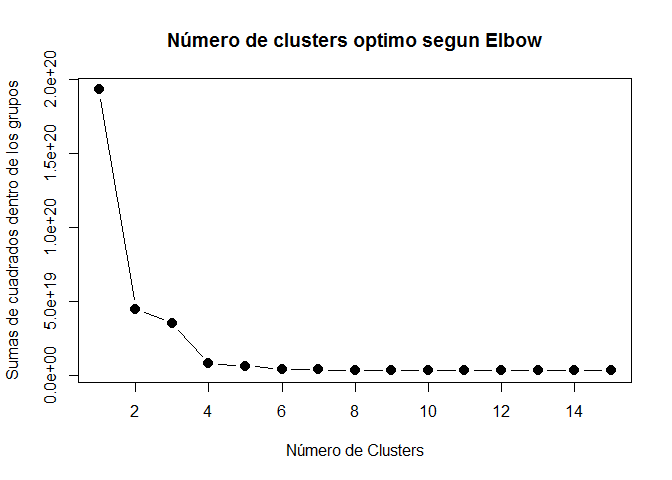
\includegraphics[width=2.5in,clip,keepaspectratio]{./model_no_supervised_files/figure-markdown_github/unnamed-chunk-2-1}
\end{figure}

En la siguiente imagen se puede ver la relación entre los distintos clusters generados según el número óptimo calculado previamente, que en este caso es 4:

\begin{figure}[h]
\centering
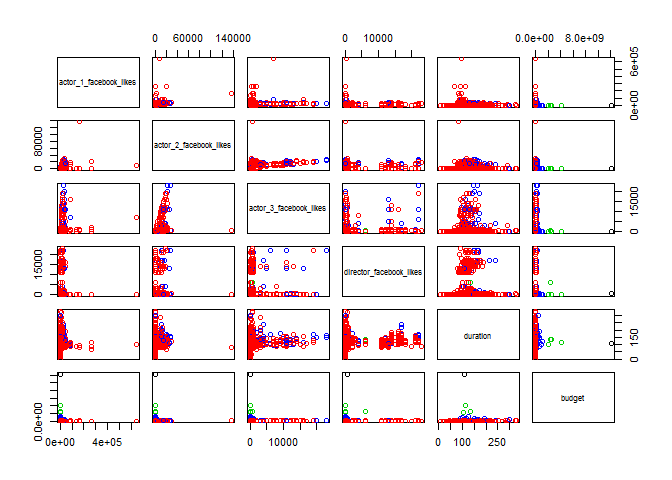
\includegraphics[width=5in,clip,keepaspectratio]{./model_no_supervised_files/figure-markdown_github/unnamed-chunk-2-2}
\end{figure}

\clearpage

\section{Modelos de Machine Learning supervisados}

Para la creación del modelo no supervisado se utilizará el conjunto de datos generado anteriormente y se calculará el número óptimo de clusters según \href{https://github.com/pozueco/proyecto_fin_de_master/blob/master/model_supervised.md}{R Markdown}:

\begin{figure}[h]
\centering
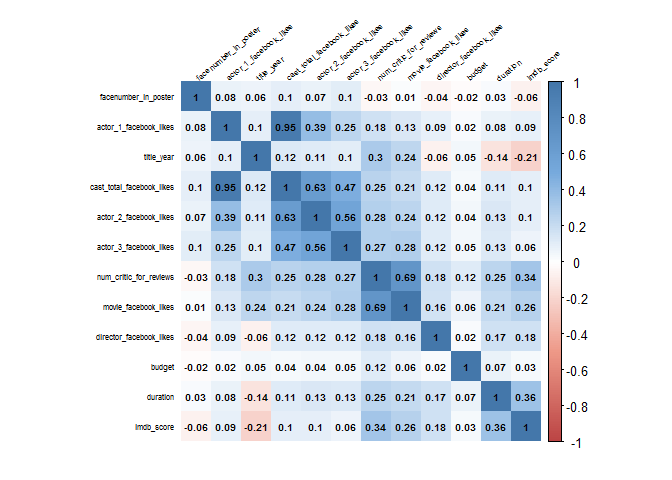
\includegraphics[width=6in,clip,keepaspectratio]{./model_supervised_files/figure-markdown_github/unnamed-chunk-3-1}
\end{figure}

\clearpage

Según la matriz de correlación anterior, existe una gran influencia entre los atributos Cast Total Facebook Likes y Actor 1 Facebook Likes, por lo que se ha eliminado esta primera para la construcción de los siguientes modelos de regresión.

El primero de ellos será un modelo de regresión Ridge\cite{glmnet} el cual será optimizado para obtener los mejores parámetros que minimicen el error del modelo obtenido con \href{https://github.com/pozueco/proyecto_fin_de_master/blob/master/model_supervised.md}{R Markdown}:


\begin{figure}[h]
\centering
\subfigure[Número de likes de los actores]{
\centering
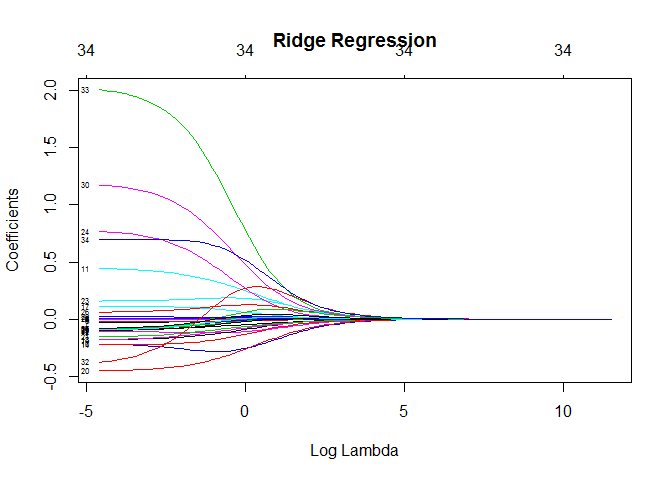
\includegraphics[width=2.6in]{./model_supervised_files/figure-markdown_github/unnamed-chunk-6-1}
}
\subfigure[Número de likes de los directores]{
\centering
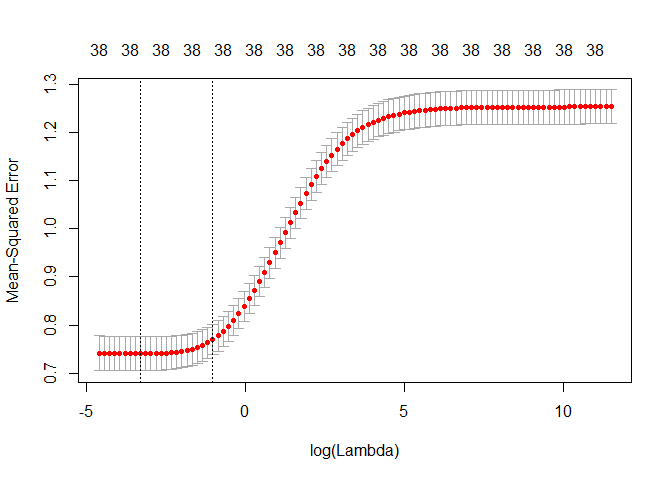
\includegraphics[width=2.6in]{./model_supervised_files/figure-markdown_github/unnamed-chunk-6-2}
}
\end{figure}

El segundo de ellos será un modelo de regresión Lasso\cite{glmnet} el cual también será optimizado para obtener los mejores parámetros que minimicen el error del modelo obtenido con \href{https://github.com/pozueco/proyecto_fin_de_master/blob/master/model_supervised.md}{R Markdown}:

\begin{figure}[h]
\centering
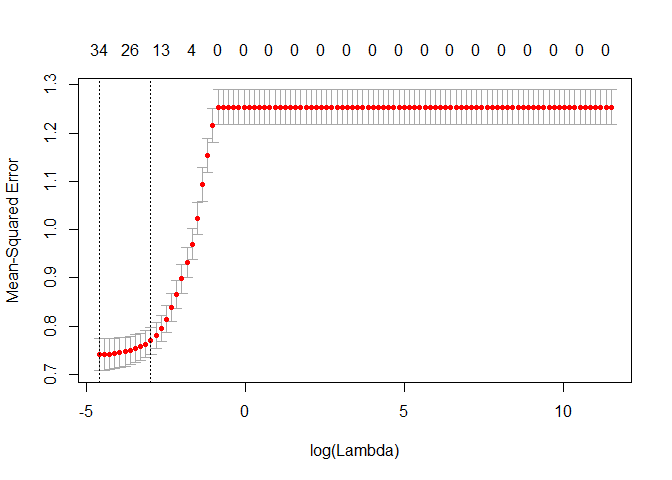
\includegraphics[width=3in,clip,keepaspectratio]{./model_supervised_files/figure-markdown_github/unnamed-chunk-7-1}
\end{figure}

\clearpage

\section{Creación de un sistema de recomendación}

\blindtext

\clearpage

\section{Conclusiones y próximos pasos}

\blindtext

\clearpage

\begin{thebibliography}{1}

%\bibitem{IEEEhowto:kopka}
%H.~Kopka and P.~W. Daly, \emph{A Guide to \LaTeX}, 3rd~ed.\hskip 1em plus
%  0.5em minus 0.4em\relax Harlow, England: Addison-Wesley, 1999.

\bibitem{imdb5000}
C.~Sun, \emph{IMDB 5000 Movie Dataset}, \href{https://www.kaggle.com/deepmatrix/imdb-5000-movie-dataset}{5000+ movie data scraped from IMDB website}, \relax Kaggle, 2016.

\bibitem{quora}
Z.~Brown, \href{https://www.quora.com/How-many-films-are-produced-each-year}{How many films are produced each year?}, \relax Quora, 2016.

\bibitem{popmatters}
M.~Lanzagorta, \href{http://www.popmatters.com/column/horror-cinema-by-the-numbers/}{Horror Cinema By the Numbers}, \relax PopMatters, 2007.

\bibitem{justgeek}
Z.~Brown, \href{http://www.justgeek.de/watching-all-the-movies-ever-made/}{Watching all the movies ever made}, \relax Justgeek, 2014.

\bibitem{glmnet}
T.~Hastie and J.~Qian, \href{https://web.stanford.edu/~hastie/glmnet/glmnet_alpha.html}{Glmnet Vignette}, \relax Stanford University, 2014.

\end{thebibliography}

% biography section
%
% If you have an EPS/PDF photo (graphicx package needed) extra braces are
% needed around the contents of the optional argument to biography to prevent
% the LaTeX parser from getting confused when it sees the complicated
% \includegraphics command within an optional argument. (You could create
% your own custom macro containing the \includegraphics command to make things
% simpler here.)
%\begin{biography}[{\includegraphics[width=1in,height=1.25in,clip,keepaspectratio]{mshell}}]{Michael Shell}
% or if you just want to reserve a space for a photo:

%\begin{IEEEbiography}[{
\includegraphics[width=1in,height=1.25in,clip,keepaspectratio]{picture}%}]{John Doe}
%%\blindtext
%\end{IEEEbiography}

% You can push biographies down or up by placing
% a \vfill before or after them. The appropriate
% use of \vfill depends on what kind of text is
% on the last page and whether or not the columns
% are being equalized.

%\vfill

% Can be used to pull up biographies so that the bottom of the last one
% is flush with the other column.
%\enlargethispage{-5in}

% that's all folks

\clearpage

\appendix

\newgeometry{left=2.5cm,right=2.5cm,top=2cm,bottom=2.5cm,footnotesep=0.5cm}

\section{Calidad del dataset} \label{anexo:I}

\begin{figure}[h]
\centering
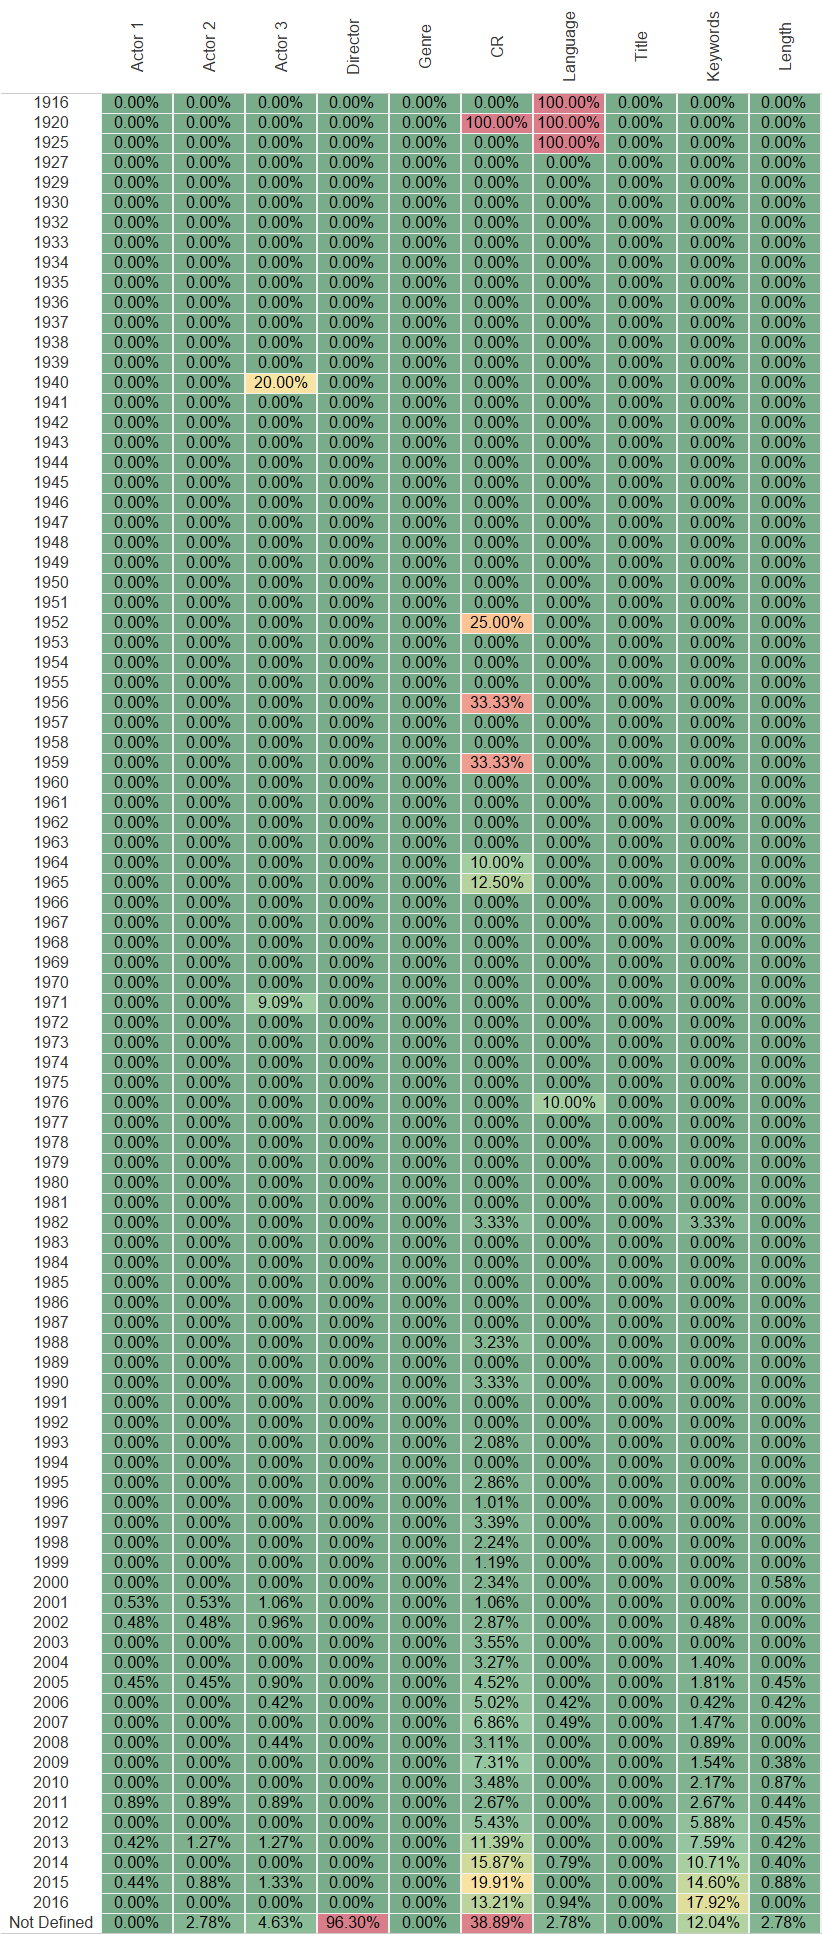
\includegraphics[height=0.78\textheight,clip,keepaspectratio]{./images/dataset_quality_dimensions}
\label{fig:imdb_num_films_per_year}
\end{figure}

\clearpage

\begin{figure}[h]
\centering
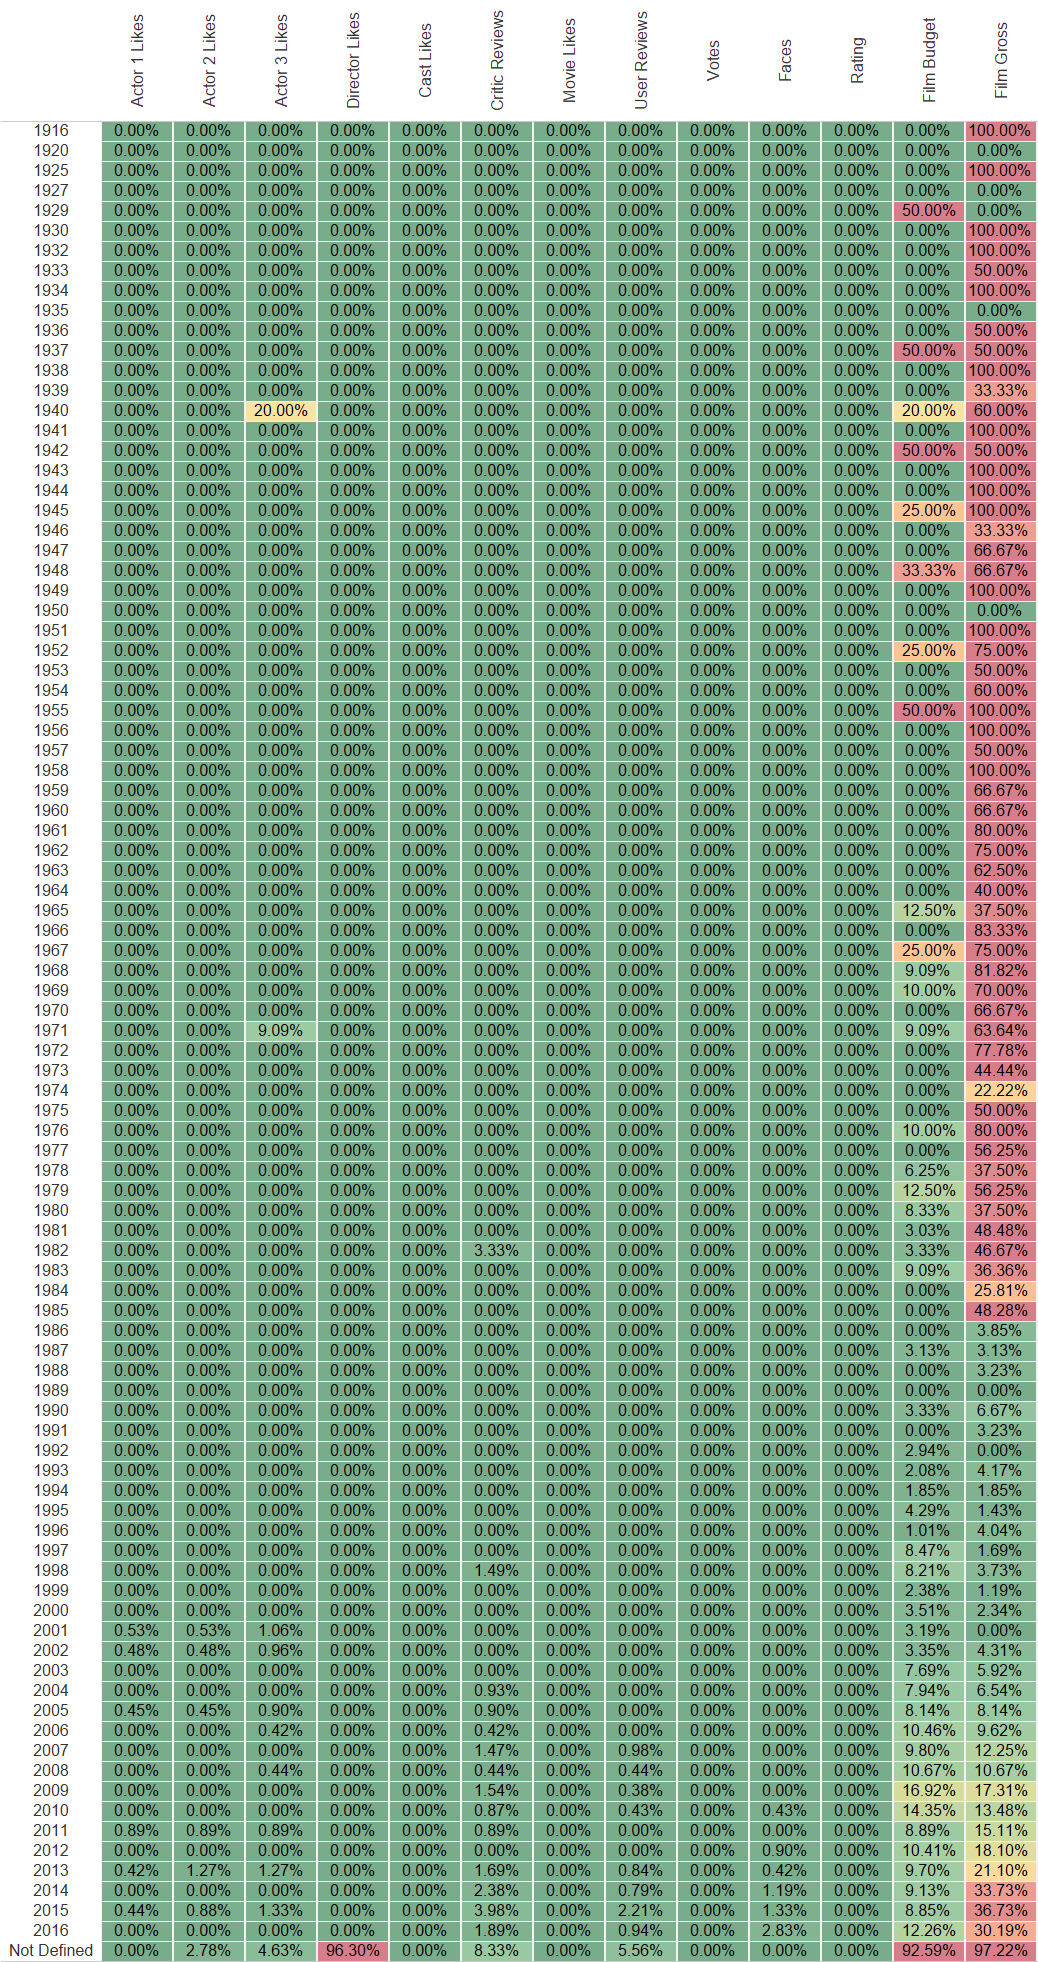
\includegraphics[height=0.78\textheight,clip,keepaspectratio]{./images/dataset_quality_metrics}
\label{fig:imdb_num_films_per_year}
\end{figure}

\end{document}
